\documentclass{standalone}
\usepackage{graphicx}	
\usepackage{amssymb, amsmath}
\usepackage{color}

\usepackage{tikz}
\usetikzlibrary{intersections, backgrounds, math}
\usepackage{pgfmath}

\definecolor{light}{RGB}{220, 188, 188}
\definecolor{mid}{RGB}{185, 124, 124}
\definecolor{dark}{RGB}{143, 39, 39}
\definecolor{highlight}{RGB}{180, 31, 180}
\definecolor{gray10}{gray}{0.1}
\definecolor{gray20}{gray}{0.2}
\definecolor{gray30}{gray}{0.3}
\definecolor{gray40}{gray}{0.4}
\definecolor{gray60}{gray}{0.6}
\definecolor{gray70}{gray}{0.7}
\definecolor{gray80}{gray}{0.8}
\definecolor{gray90}{gray}{0.9}
\definecolor{gray95}{gray}{0.95}


\begin{document}

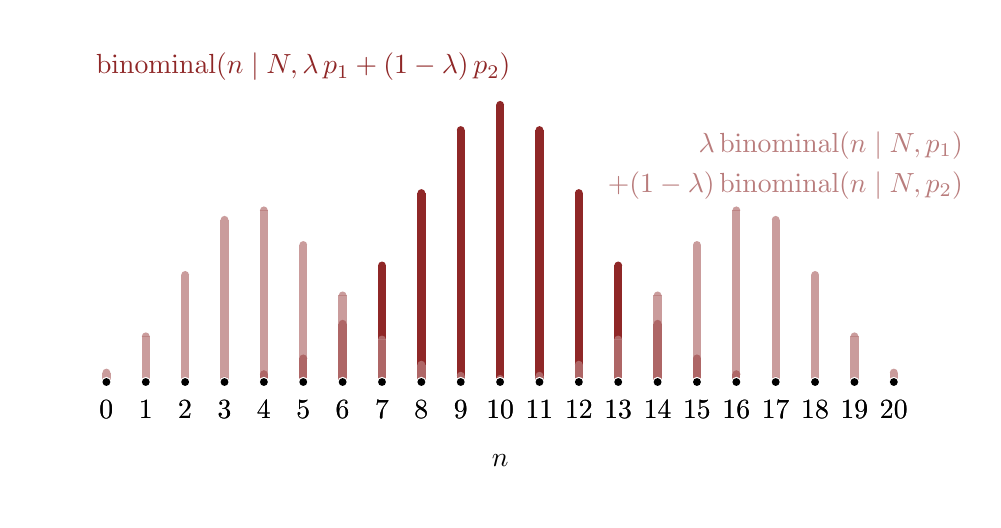
\begin{tikzpicture}[scale=1]
  \begin{scope}[shift={(0, 0)}]
    \fill[white] (-6, -3.5) rectangle (6, 2.5);
   
    \foreach [count=\n] \m in {0.000, 0.000, 0.000, 0.001, 0.005, 0.015, 0.037, 0.074, 
                               0.120, 0.160, 0.176, 0.160, 0.120, 0.074, 0.037, 0.015, 
                               0.005, 0.001, 0.000, 0.000, 0.000} {
      \pgfmathsetmacro{\x}{0.5 * ( (\n - 1) - 10)};
      \draw[dark, line width=3] (\x, -2) -- (\x, {(20 * \m - 2)});
      \fill[dark] (\x, {(20 * \m - 2)}) circle (0.05);
      \fill[white] (\x, -2) circle (0.065);
      \fill[black] (\x, -2) circle (0.05);
      
      \pgfmathtruncatemacro{\nn}{\n - 1}
      \node at (\x, -2.35) { $\nn$ };
    }
    
    \node[dark] at (-2.5, 2) { $\mathrm{binominal}(n \mid N, \lambda \, p_{1} + (1 - \lambda) \, p_{2})$ };
 
    \foreach [count=\n] \m in {0.006, 0.029, 0.068, 0.103, 0.109, 0.087, 0.055, 0.027, 
                               0.011, 0.004, 0.002, 0.004, 0.011, 0.027, 0.055, 0.087, 
                               0.109, 0.103, 0.068, 0.029, 0.006} {
      \pgfmathsetmacro{\x}{0.5 * ( (\n - 1) - 10 )};
      \pgfmathsetmacro{\y}{20 * \m - 2};
      \draw[mid, opacity=0.75, line width=3] (\x, -2) -- (\x, \y);
      
      \begin{scope}
        \clip (\x - 0.1, \y) rectangle (\x + 0.1, \y + 0.1);
        \fill[mid, opacity=0.75] (\x, \y) circle (0.05);
      \end{scope}
      
      \fill[white] (\x, -2) circle (0.065);
      \fill[black] (\x, -2) circle (0.05);
      
      \pgfmathtruncatemacro{\nn}{\n - 1}
      \node at (\x, -2.35) { $\nn$ };
    }
    
    \node[mid, anchor=east] at (6, 1.00) { $\lambda \, \mathrm{binominal}(n \mid N, p_{1})$ };
    \node[mid, anchor=east] at (6, 0.50) { $+ (1 - \lambda) \, \mathrm{binominal}(n \mid N, p_{2})$ };
 
    \node at (0, -3) { $n$ };
  \end{scope}
  
\end{tikzpicture}

\end{document}  